\documentclass{article}
\usepackage[T1]{fontenc}
\usepackage{lmodern}
\usepackage[polish]{babel}
\usepackage{graphicx}
\usepackage{float}
\usepackage{hyperref}

\usepackage[a4paper, margin=2.54cm]{geometry}

\title{Raport skuteczności lasów losowych}
\author{Maciej Szefler, Kacper Karski,
    \\Damian Jankowski, Filip Krawczak}

\begin{document}

\maketitle

\tableofcontents

\section{Wstęp}

Las losowy (ang. Random Forest) to algorytm uczenia maszynowego, który jest używany zarówno do zadań klasyfikacji, jak i regresji. Jest to przykład metody która polega na łączeniu wyników wielu modeli bazowych w celu uzyskania lepszej ogólnej wydajności. Działanie tego algorytmu polega na losowym wyborze podzbiorów danych z zestawu treningowego. Każde drzewo jest trenowane na innym podzbiorze danych, co wprowadza losowość i różnorodność w procesie uczenia. Podczas budowy każdego drzewa, losowo wybiera się tylko pewną liczbę cech spośród wszystkich dostępnych cech. Ten proces pomaga w zwiększeniu różnorodności modeli i unika przewagi nadmiernie wpływających cech. Następnie w przypadku klasyfikacji, algorytm Lasu Losowego przewiduje wynik na podstawie głosowania drzew, wybierając najczęściej występującą klasę. W przypadku regresji, przewiduje się średnią wartość przewidywaną przez wszystkie drzewa. Dzięki losowym podzbiorom danych i cech oraz kombinacji wielu drzew, Las Losowy jest generalnie mniej podatny na przeuczenie (ang. overfitting) niż pojedyncze drzewo decyzyjne. Różnorodność drzew pomaga w zwiększeniu ogólnej zdolności do generalizacji modelu.  Przewagą algorytmu lasu losowego jest jego wysoka skuteczność w stosunku do relatywnie niskiej ilości próbek.

Wykorzystany algorytm lasu losowego klasyfikuje znormalizowane dane związane z oddechem. Algorytm jest używany do przewidywania trzech stanów: bezdech, wdech i wydech, na podstawie otrzymanych 5 próbek, dla których określa stan oddechu. Sklasyfikowane dane następnie są przekazywane jako dane treningowe do modelu sieci neuronowej. Cały proces można określić jako uproszczony Transfer Labelling. Algorytm Lasu Losowego działa jako etap wstępny do etapu uczenia sieci neuronowej, co prowadzi do lepszych wyników klasyfikacji danych związanych z oddechem.


\section{Forest Model}

\begin{figure}[H]
    \centering
    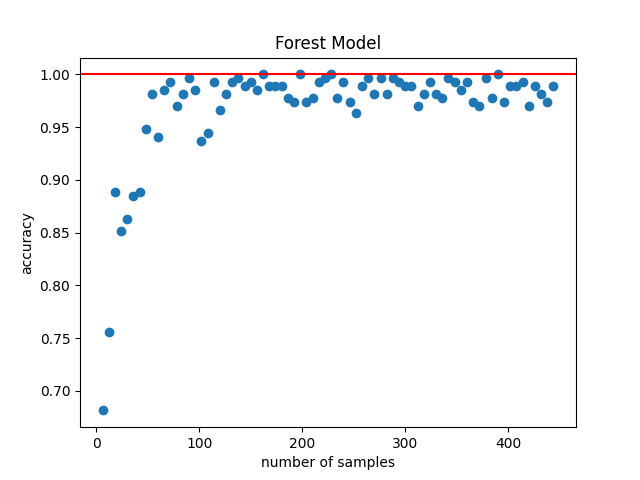
\includegraphics[width=0.75\textwidth]{transfer_labelling_forest.png}
    \caption{Skuteczność lasu losowego w zależności od liczby próbek treningowych}
\end{figure}

Wykres przedstawia zależność między liczbą próbek a dokładnością modelu lasów losowych. Punkty na wykresie reprezentują dokładność modelu dla różnych liczb próbek użytych do treningu. Linia pozioma wskazuje na wartość dokładności równej 1.00, która jest teoretycznym maksimum.

Na podstawie rozproszenia punktów można zaobserwować, że dokładność modelu generalnie wzrasta wraz z liczebnością próbek, osiągając stabilizację blisko maksymalnej możliwej wartości dokładności. Większość punktów koncentruje się w górnej części wykresu, powyżej wartości dokładności 0.95, co wskazuje na wysoką wydajność modelu.

Jednakże, istnieje kilka punktów, które odstają od ogólnej tendencji, gdzie dokładność jest znacząco niższa, szczególnie przy mniejszej liczbie próbek. Te anomalie mogą wskazywać na przypadki, w których model miał trudności z generalizacją na skutek ograniczonej ilości danych lub specyficznych cech danych treningowych.

Podsumowując, przedstawione dane sugerują, że model lasów losowych osiąga wysoką dokładność w zadaniu klasyfikacyjnym, przy czym efektywność ta stabilizuje się przy większej liczbie próbek. Odstające wartości w dolnej części wykresu, mimo że są w mniejszości, mogą wymagać dodatkowej analizy, aby zrozumieć przyczyny niższej dokładności w tych przypadkach. Wyniki te wskazują na potencjalną potrzebę dalszej optymalizacji procesu treningowego lub przeglądu metody selekcji i przetwarzania próbek treningowych.

Dane otagowane przez model Lasu Losowego zostały wykorzystane do nauczenia modeli sieci neuronowych.

\begin{figure}[H]
    \centering
    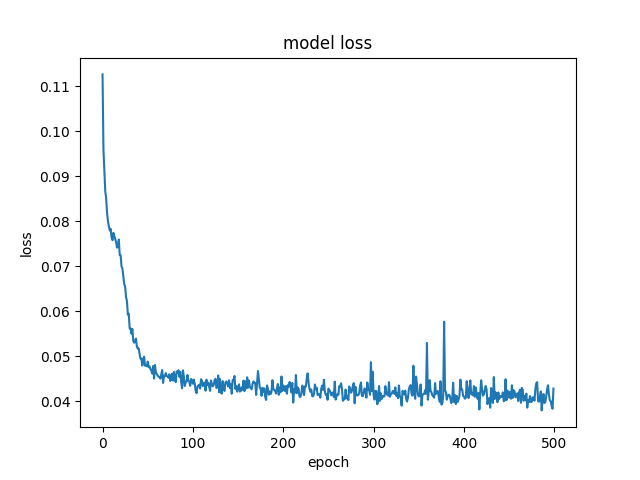
\includegraphics[width=0.75\textwidth]{epoch_loss_forest.png}
    \caption{Krzywa strat modelu lasów losowych}
\end{figure}

Wykres przedstawia zmianę funkcji straty modelu w zależności od liczby epoch w procesie uczenia. Widać, że wartość straty modelu gwałtownie spada w początkowej fazie uczenia, co wskazuje na szybką adaptację modelu do danych treningowych. Początkowa wartość straty znajduje się na poziomie około 0.11 i spada do około 0.05 już po niewielkiej liczbie epoch.

Po tej wstępnej fazie szybkich ulepszeń, krzywa strat wykazuje trend spadkowy, osiągając stabilizację z niewielkimi fluktuacjami wokół wartości 0.04. Pojawienie się tych fluktuacji może sugerować momenty, w których model napotykał na trudniejsze do nauki przypadki w danych lub kiedy dostosowywał się do subtelniejszych cech danych treningowych.

Na wykresie obserwujemy także pewne artefakty w wartościach strat, które występują sporadycznie po około 400 epochach. Te artefakty mogą wskazywać na przeuczenie się modelu lub na niestabilności w procesie uczenia, co mogłoby być wynikiem na przykład zbyt wysokiej stopy uczenia się lub anomalii w danych treningowych.

Podsumowując, przedstawiony wykres pokazuje typową krzywą uczenia się dla modelu maszynowego, z szybkim postępem na początku i stabilizacją w miarę zbliżania się do optymalnej wydajności. Stabilizacja wartości straty na niskim poziomie wskazuje na to, że model osiągnął zadowalający poziom generalizacji. Jednakże, obserwowane fluktuacje i artefakty mogą wymagać dalszej analizy w celu zapewnienia, że model jest dobrze dostrojony i nie występuje przeuczenie.


\section{Wyniki}

\begin{figure}[H]
    \centering
    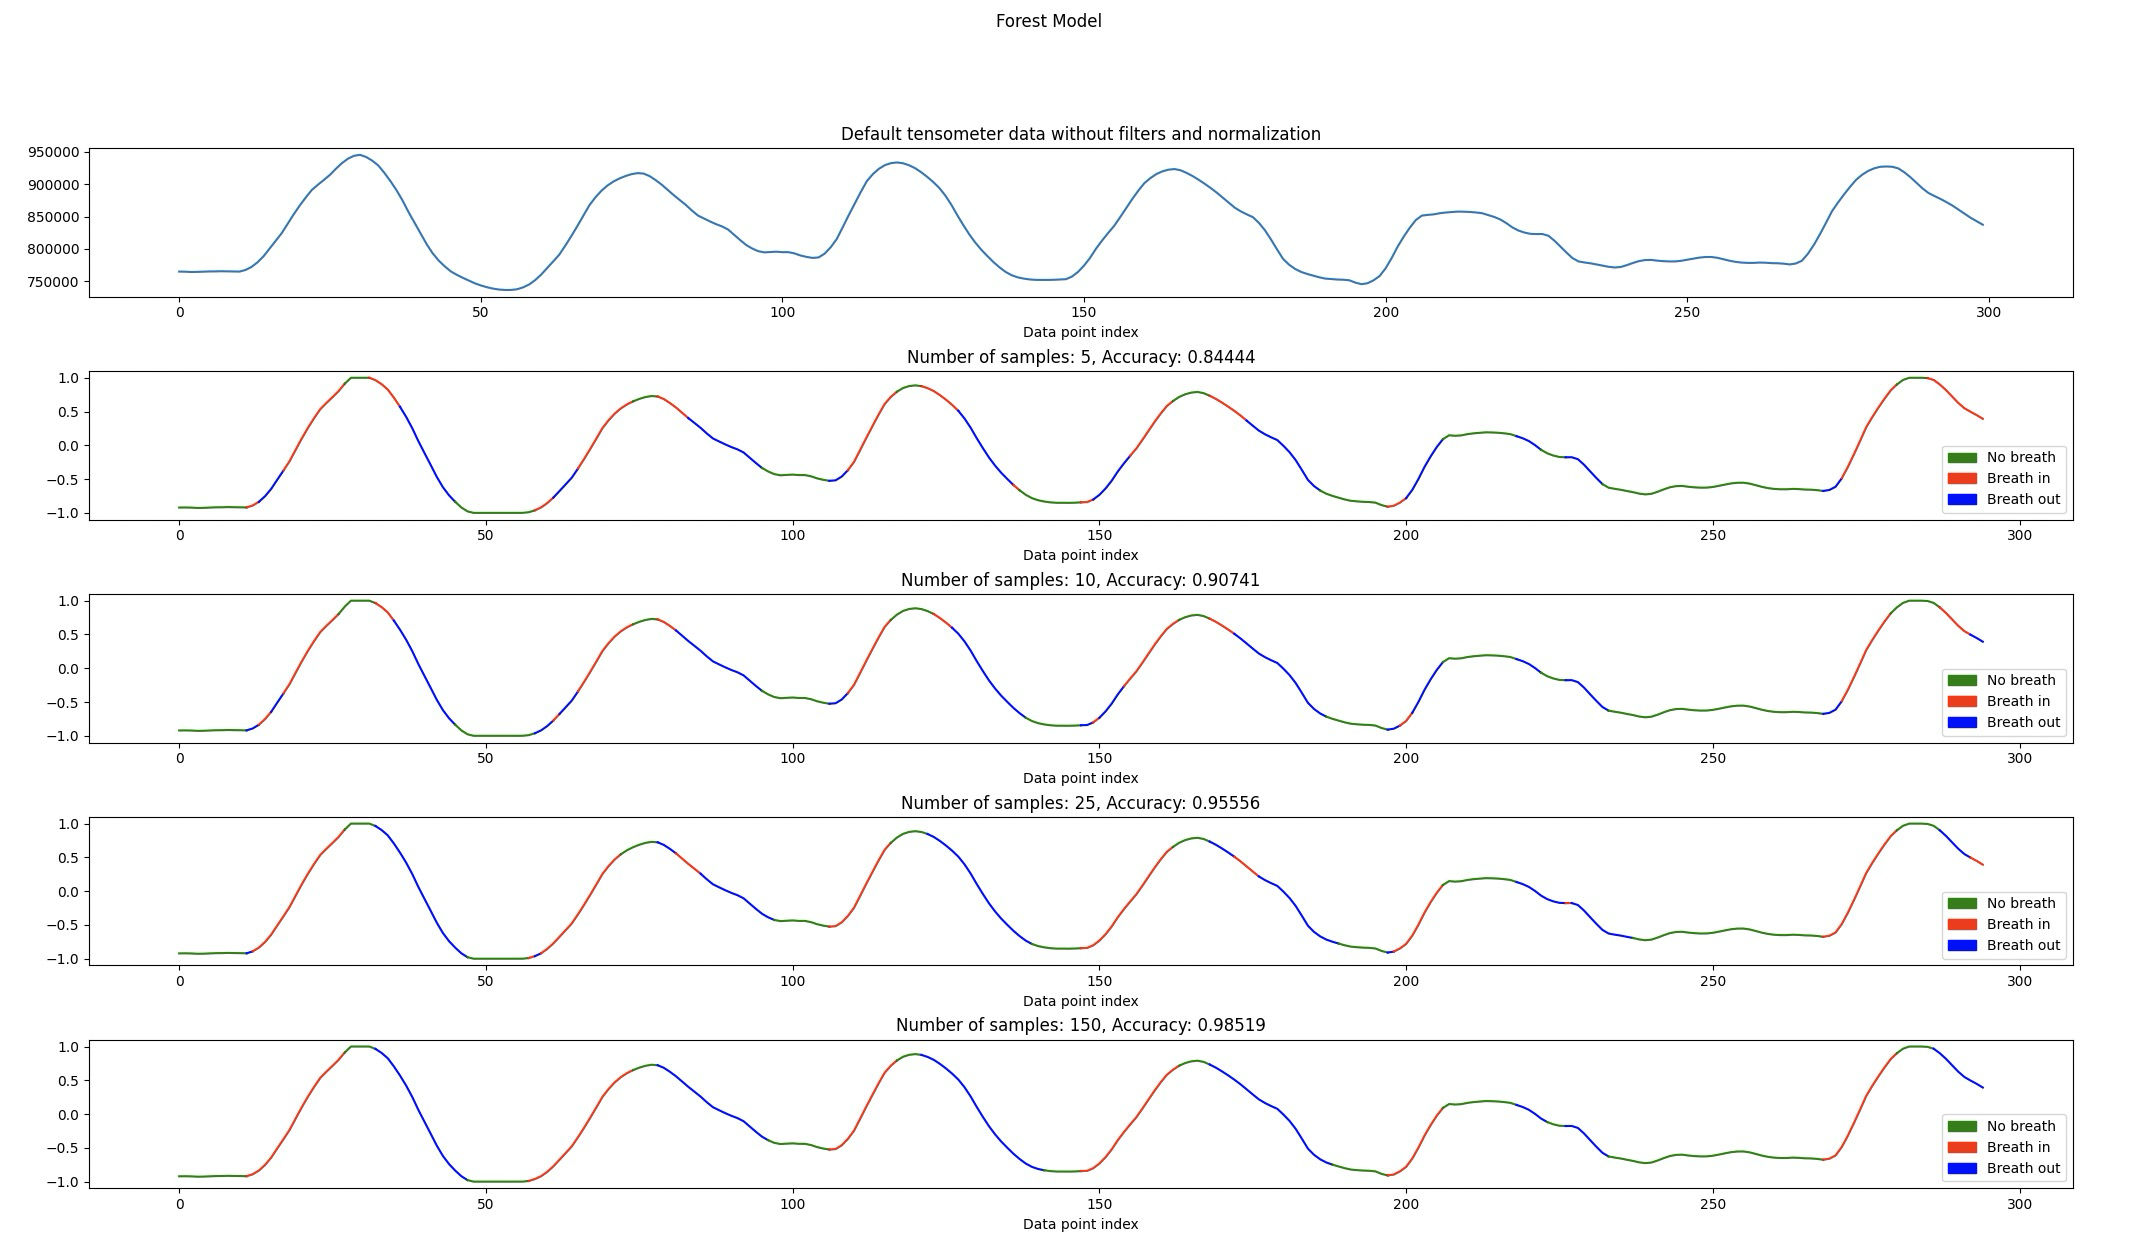
\includegraphics[width=\textwidth]{jak_sobie_radzi_las_losowy.png}
    \caption{Skuteczność lasu losowego od liczby próbek treningowych dla 300 próbek testowych}
\end{figure}

\begin{figure}[H]
    \centering
    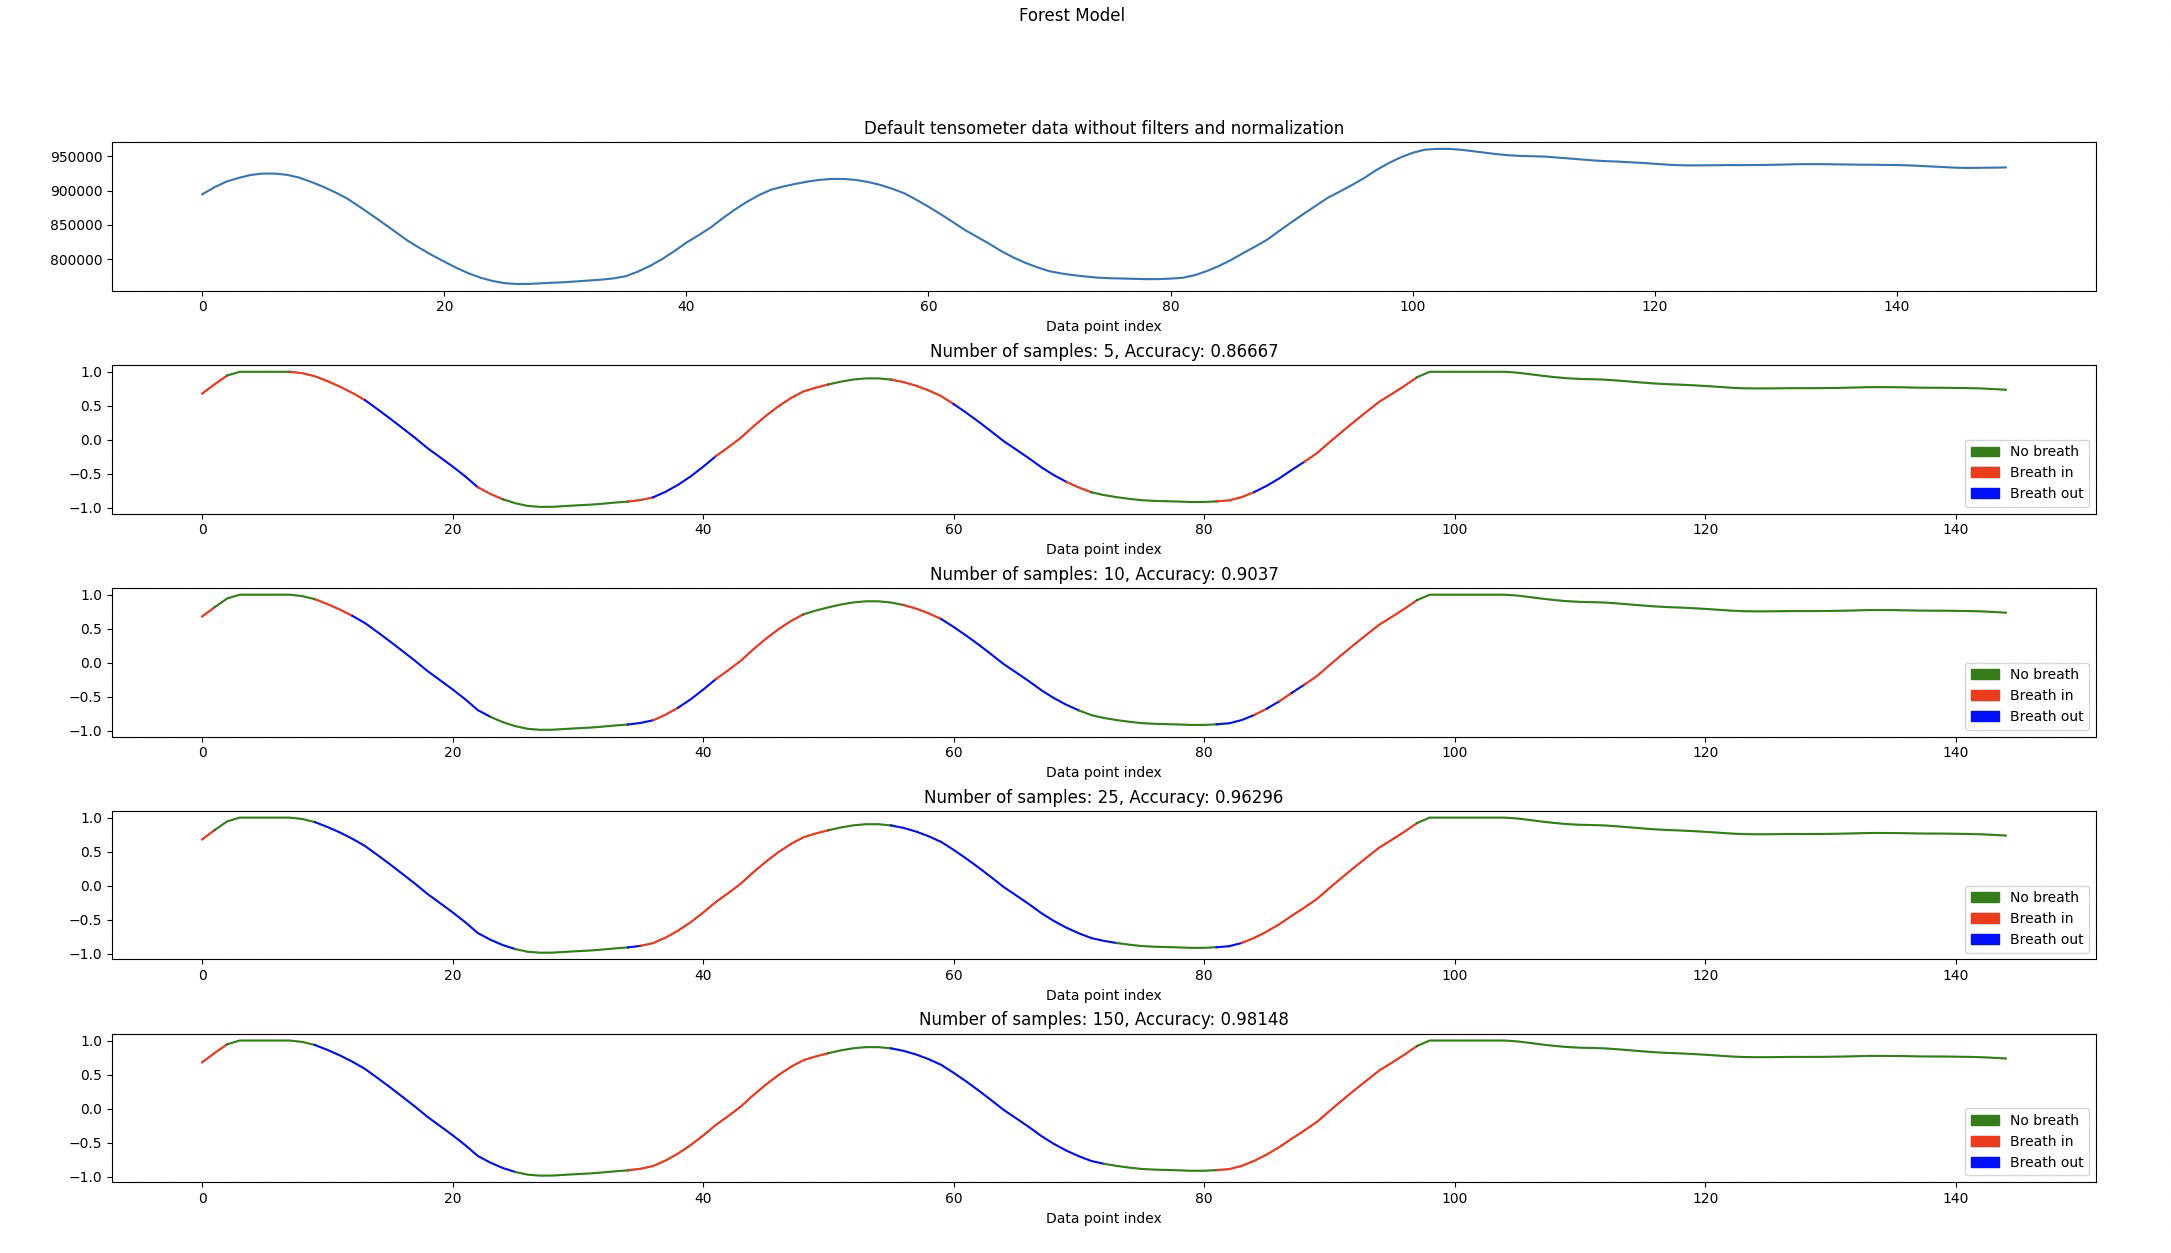
\includegraphics[width=\textwidth]{jak_sobie_radzi_las_losowy_2.png}
    \caption{Skuteczność lasu losowego od liczby próbek treningowych dla 150 próbek testowych}
\end{figure}

Przedstawione wykresy ilustrują efektywność modelu w zależności od liczby próbek wykorzystanych do treningu. Pierwszy wykres w sekwencji nie zawiera danych klasyfikacyjnych, służąc jako odniesienie do zestawu danych wejściowych bez zastosowania filtrów i normalizacji.

W kolejnych eksperymentach, gdzie liczba próbek wykorzystanych do treningu wynosi odpowiednio 5, 10, 25 i 150 (ilość próbek dla każdego stanu), obserwujemy progresywną poprawę dokładności klasyfikacji od wartości $\sim$0.85 do $\sim$0.985. Wzrost dokładności jest korelowany z zwiększającą się liczbą próbek treningowych, co jest zgodne z powszechnie akceptowanymi założeniami w dziedzinie uczenia maszynowego. Dane te sugerują, że model Random Forest wykazuje zdolność do generalizacji i poprawy wyników przy większej objętości danych treningowych.

Analizując przedstawione wykresy, można zauważyć że modele uczone na mniejszej liczbie próbek, słabo radzą sobie w momentach zaszumienia sygnałów. Szczególnie warto zwrócić uwagę na momenty zmian stanów. W takich sytuacjach, modele uczone na mniejszej liczbie próbek, niepoprawnie klasyfikują dane.

Rezultaty te mogą mieć znaczące implikacje dla monitorowania parametrów życiowych w realnym czasie, szczególnie w kontekście detekcji i analizy oddechu. Wysoka dokładność modelu przy wyższej liczbie próbek treningowych wskazuje na jego potencjalną przydatność w zastosowaniach klinicznych oraz w systemach wspierających decyzje medyczne.


\end{document}